%哈尔滨商业大学本科生论文latex模板
%@Version : 1.0  
%@Time    : 2018/11/9
%@Author  : 冷冠男
%非常感谢华东师范大学的袁轶军同学,解决了我很多的问题与疑惑
%欢迎同学们提出建议与论文的错误,我会及时更改

\documentclass[a4paper,oneside,UTF8]{article} %A4纸,单面,UTF-8

\usepackage{fancybox,fancyvrb,shortvrb} %也许需要的宏包
\usepackage[heading]{ctex} %用来提供中文支持
\usepackage{amsmath} %
\usepackage{amssymb} %数学符号,定理等环境相关宏包
\usepackage{amsthm}  %
\usepackage{graphicx} %插入图片所需宏包
\usepackage{adjustbox}  %也许需要的宏包
\usepackage{xspace} %提供一些好用的空格命令
\usepackage{tikz-cd} %画交换图需要的宏包
\usepackage{url} %更好的超链接显示
\usepackage{array} %表格相关的宏包
\usepackage{booktabs} %表格相关的宏包
\usepackage{caption} %实现图片的多行说明
\usepackage{float} %图片与表格的更好排版
\usepackage{ifthen}%这个宏包提供逻辑判断命令
\newboolean{first}%定义一个布尔变量用于判断是否为首页
\setboolean{first}{true}%设定fist变量初值为true
\usepackage{lastpage}                                           
\usepackage{layout}
\usepackage{pdfpages}
\usepackage{cite}

\usepackage{titletoc}%使所有目录后都有引导点
\titlecontents{section}[0pt]{\addvspace{2pt}\filright}
{\contentspush{\thecontentslabel\ }}
{}{\titlerule*[8pt]{.}\contentspage}
%==========================================================
%图标公式按章节显示
\renewcommand {\thetable} {\thesection{}.\arabic{table}}
\renewcommand {\thefigure} {\thesection{}.\arabic{figure}}
\renewcommand{\theequation}{\arabic{section}-\arabic{equation}}
\DeclareCaptionFont{zhten}{\songti\zihao{5}\selectfont}%设置图表字体为宋体五号
\captionsetup{font = zhten}
\captionsetup{labelsep=quad}%冒号换为一个空格

\usepackage{ulem} %更好的下划线

\usepackage[ top=3.5cm, bottom=2.5cm, left=3.0cm, right=2.5cm]{geometry} %设置页边距

\usepackage{fontspec}                   %设置字体需要的宏包
\setmainfont{Times New Roman}           %设置西文字体为Times New Roman
\setCJKmainfont{SimSun}                 %设置中文字体为宋体
\renewcommand{\normalsize}{\zihao{-4}\setlength{\baselineskip}{20pt}}  %设置正文字号为小四
\linespread{1.5} %1.5倍行距
\showboxdepth=5
\showboxbreadth=5 
\setcounter{secnumdepth}{5}                                                                                     %
\ctexset { section = { name={,},format={\centering \heiti \zihao {-2}\setlength{\baselineskip}{20pt}} } }         %
\ctexset { subsection = { name={,},format={\heiti \zihao {-3}\setlength{\baselineskip}{20pt}} } } %设置各级系统的编号格式
\ctexset { subsubsection = { name={,},format={\heiti \zihao {4}\setlength{\baselineskip}{20pt}} } }          %
\ctexset { paragraph = { name={,},format={\heiti \zihao {-4}} } }               %
\ctexset { subparagraph = { name={,},format={\heiti \zihao {-4}} } }           %

\usepackage[bottom,perpage]{footmisc}               %脚注,显示在每页底部,编号按页重置
\renewcommand*{\footnotelayout}{\zihao{-5}\songti}  %设置脚注为小五号宋体
\renewcommand{\thefootnote}{[\arabic{footnote}]}    %设置脚注标记为  [编号]
                      %脚注的反向超链接

\usepackage{fancyhdr}               %

%\renewcommand{\headrulewidth}{0pt}  %
%\lhead{哈尔滨商业大学学士学位论文}                            %
%\chead{}                            %将页眉页脚设置为:仅在右下角显示页码
%\rhead{\TitleCHS}                            %
%\lfoot{}                            %
\cfoot{\thepage}                            %
%\rfoot{\thepage}                    %

\lhead{}
\chead{哈尔滨商业大学本科毕业设计(论文)}{\zihao{5}\songti}
\rhead{}
%%=====================================================
%%双线页眉的设置
\makeatletter %双线页眉
\def\headrule{{\if@fancyplain\let\headrulewidth\plainheadrulewidth\fi%
		\hrule\@height 2.276pt \@width\headwidth\vskip1pt%上面线为1pt粗
		\hrule\@height 0.4pt\@width\headwidth  %下面0.5pt粗
		\vskip-2\headrulewidth\vskip-1pt}      %两条线的距离1pt
	\vspace{6mm}}     %双线与下面正文之间的垂直间距
\makeatother

\usepackage{xcolor} %彩色的文字

\usepackage[hidelinks]{hyperref} %各种超链接必备

\usepackage{footnotebackref}  


\newtheorem{theorem}{\heiti 定理}[section]      %
\newtheorem*{theorem*}{\heiti 定理}             %
\newtheorem{lemma}[theorem]{\heiti 引理}        %
\newtheorem*{lemma*}{\heiti 引理}               %
\newtheorem{corollary}[theorem]{\heiti 推论}    %
\newtheorem*{corollary*}{\heiti 推论}           %
\newtheorem{definition}[theorem]{\heiti 定义}   %
\newtheorem*{definition*}{\heiti 定义}          %
\newtheorem{conjecture}[theorem]{\heiti 猜想}   %将各种常用环境设置为中文
\newtheorem*{conjecture*}{\heiti 猜想}          %
\newtheorem{problem}[theorem]{\heiti 问题}      %
\newtheorem*{problem*}{\heiti 问题}             %
\newenvironment{solution}                       %
  {\renewcommand\qedsymbol{$\blacksquare$}      %
  \begin{proof}[\heiti \bf 解]}                 %
  {\end{proof}}                                 %
\renewcommand*{\proofname}{\heiti \bf 证明}     %

\allowdisplaybreaks %允许公式跨页显示

\clearpage

\newcommand{\makeapdx}{
	\clearpage
	%%\apdx{附录}
%%23333333333333333333333333333333333333333
%
%\apdx{调查结果}
%23333333333333333333333333333333333333333


\begin{appendix}
	\section*{附录1}
	x
	\clearpage
	\section*{附录2}
	y
\end{appendix}
}

\newcommand{\makeacknowledgement}{	 %
\clearpage                           %生成感谢,请勿改动
\input{./ending/acknowledgement.tex} %
}                                    %

%For Algorithm
\usepackage{algorithm}
\usepackage{algorithmicx}
\usepackage{algpseudocode}
\floatname{algorithm}{算法}
\renewcommand{\algorithmicrequire}{\textbf{输入:}}
\renewcommand{\algorithmicensure}{\textbf{输出:}}
\usepackage{bm}


%可能会需要在用自然语言描述算法步骤时使用的宏包
\usepackage{enumitem}

%表格单元格内换行
\newcommand{\tabincell}[2]{\begin{tabular}{@{}#1@{}}#2\end{tabular}}

 %加载各宏包以及本模板的主要设置
\newcommand{\upcite}[1]{\textsuperscript{\textsuperscript{\cite{#1}}}}%在右上角显示角标
\begin{document}
%\pagestyle{empty} %不对正文前的各页面使用页眉页脚

%请不要修改本页的任何代码!
%请不要修改本页的任何代码!
%请不要修改本页的任何代码!
\thispagestyle{empty}
\begin{titlepage}
    \newcommand{\TitleCHS}{ \songti\zihao{3}  哈尔滨商业大学本科毕业设计(论文)}

\newcommand{\TitleENG}{ \heiti\zihao{-1}毕业设计(论文)题目 } %论文标题

\newcommand{\Author}{张三} %作者名字

\newcommand{\StudentID}{23333333333} %学号

\newcommand{\Department}{能建} %院系

\newcommand{\Major}{建环} %专业

\newcommand{\Class}{建环} %班级

\newcommand{\Supervisor}{李四} %导师名字

%\newcommand{\AcademicTitle}{副工程师} %导师职称

%\newcommand{\CompleteYear}{2048} %毕业年份

%\newcommand{\CompleteMonth}{3} %毕业月份

\newcommand{\KeywordsCHS}{关键词1;关键词2;关键词3;关键词4;关键词5;关键词6;关键词7 } %中文关键词

\newcommand{\KeywordsENG}{keyword1;keyword2;keyword3;keyword4;keyword5; keyword6;keyword7} %英文关键词

    \setlength\parindent{0pt} %首行不缩进

%\parbox[t][5cm][t]{\textwidth}{
%    \begin{center}
%
\includegraphics[height=2.5cm]{figures/HUC}
%    \end{center} }%图片

\parbox[t][3cm][t]{\textwidth   }{\Huge
\begin{center} {\bf \textbf \TitleCHS } \end{center} } %汉字

\parbox[t][14cm][t]{\textwidth}{\huge
\begin{center} {\bf  \TitleENG } \end{center} }%英文

    \parbox[t][5cm][c]{\textwidth}{ {\Large
    \begin{center}

    \renewcommand{\arraystretch}{1.0}

    \begin{tabular}{p{0cm}p{5em}l@{\extracolsep{1em}}l}
    ~ & 学\hfill 生\hfill 姓\hfill 名&\hfill : &  \underline{{\bf\makebox[4.5cm][c]{\Author}}}\\
    ~ & 学\hfill 号&\hfill : &  \underline{{\bf\makebox[4.5cm][c]{\StudentID}}} \\
    ~ & 指\hfill 导\hfill 教\hfill 师&\hfill : &  \underline{{\bf\makebox[4.5cm][c]{\Supervisor}}}\\
    ~ & 班\hfill 级&\hfill : &  \underline{{\bf\makebox[4.5cm][c]{\Class}}} \\
   
    ~ & 学\hfill 院&\hfill : &  \underline{{\bf\makebox[4.5cm][c]{\Department}}} \\
    \end{tabular}
%\underline{{\bf\makebox[4.5cm][c]{\Supervisor\hspace{1em}\AcademicTitle}}}   
%    ~ & 完\hfill 成\hfill 日\hfill 期 & & \underline{{\bf\makebox[4.5cm][c]{\CompleteYear 年 \CompleteMonth 月}}}\\
    \end{center}  } }
    \vfill
%\songti\zihao{3}
%{\centering
%\ctexset{today=big}         % 汉字数字形式日期
%\today     \\ % 使用最后一次编译的日期, 实现日期的自动化
%% Date:\hspace{0.5\ccwd} Month\hspace{2\ccwd} Day\hspace{1\ccwd} Year
%}
\end{titlepage}  %插入内封面
% 直接拼入外部的开题报告单页PDF
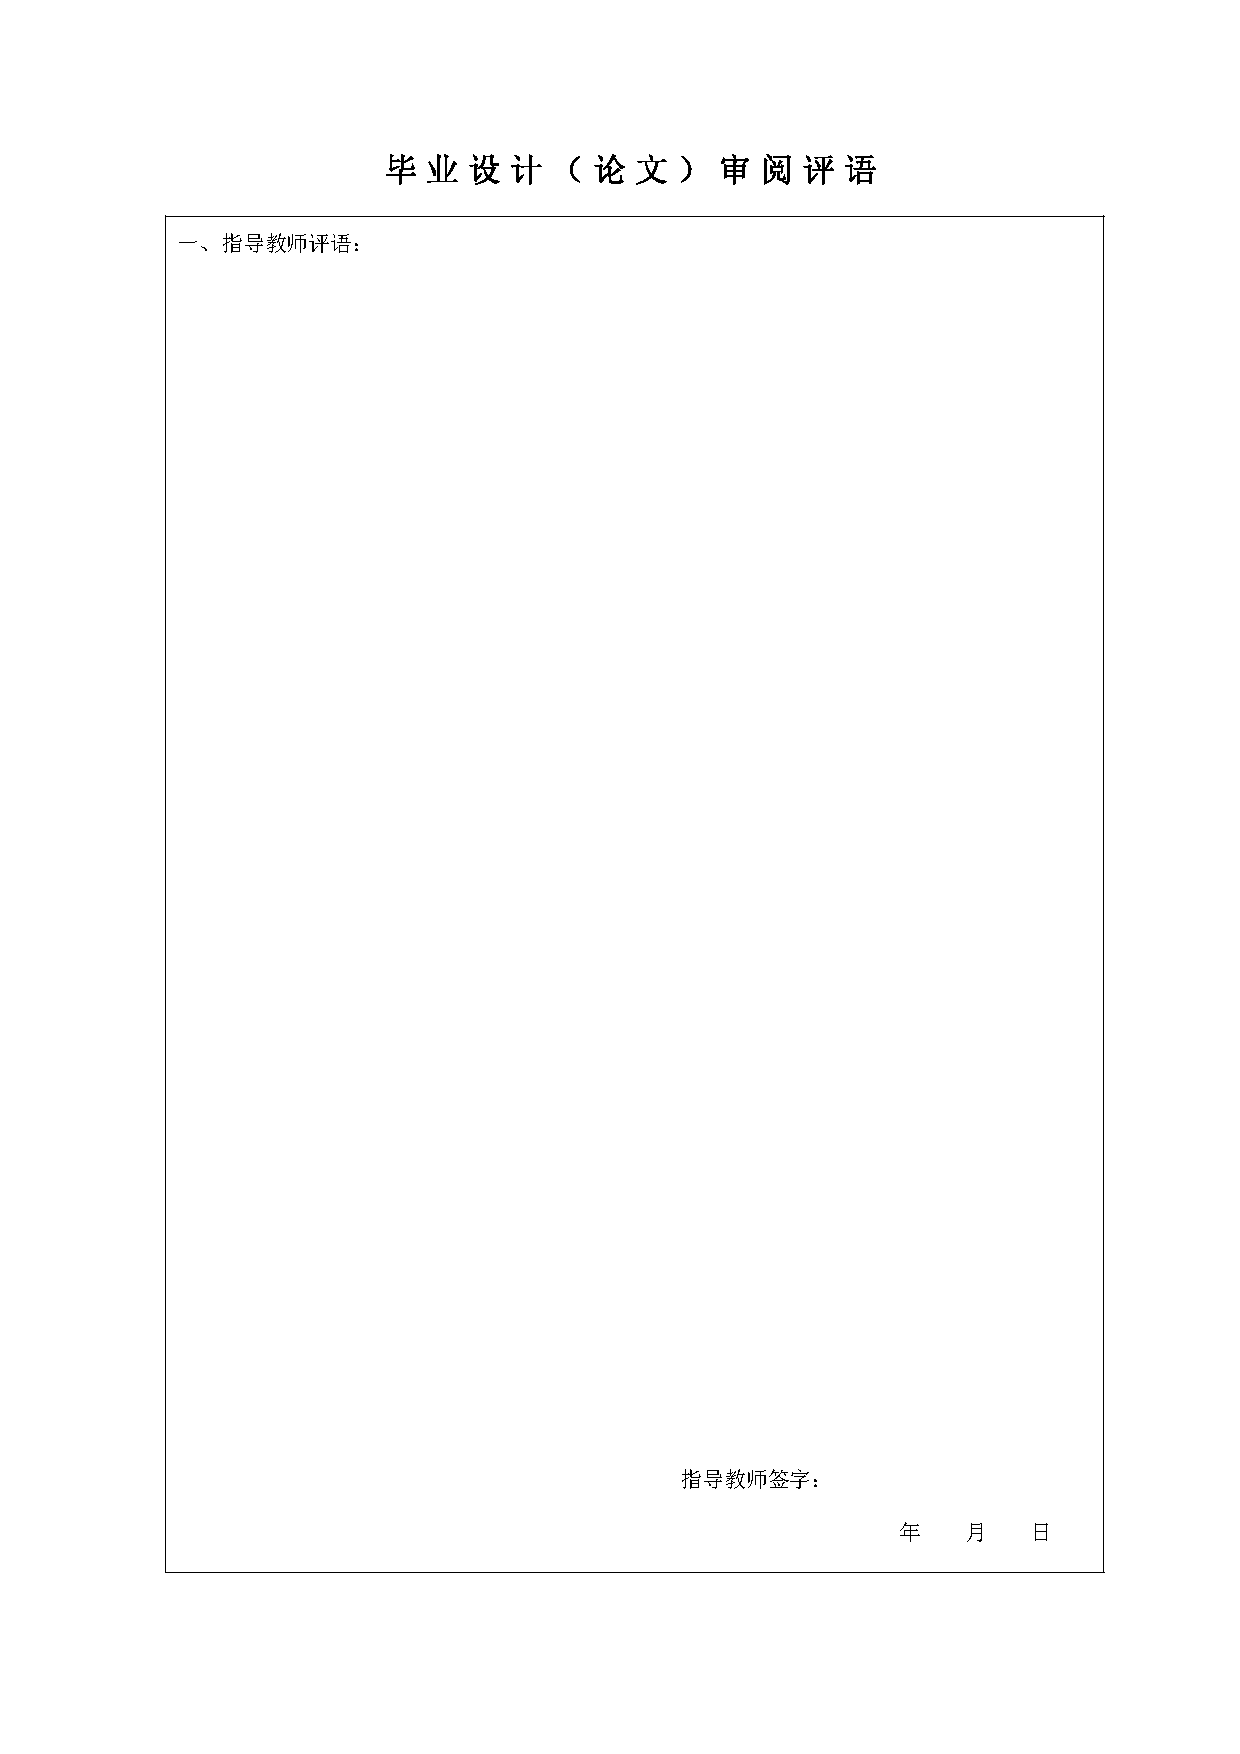
\includepdf[pages={1,2,3}]{pingyu.pdf}
\pagestyle{fancy}
\pagenumbering{Roman}%将页码变为罗马数字
\clearpage
%\pagestyle{empty}
                                          %       
                               %
\newcommand{\TitleCHS}{ \songti\zihao{3}  哈尔滨商业大学本科毕业设计(论文)}

\newcommand{\TitleENG}{ \heiti\zihao{-1}毕业设计(论文)题目 } %论文标题

\newcommand{\Author}{张三} %作者名字

\newcommand{\StudentID}{23333333333} %学号

\newcommand{\Department}{能建} %院系

\newcommand{\Major}{建环} %专业

\newcommand{\Class}{建环} %班级

\newcommand{\Supervisor}{李四} %导师名字

%\newcommand{\AcademicTitle}{副工程师} %导师职称

%\newcommand{\CompleteYear}{2048} %毕业年份

%\newcommand{\CompleteMonth}{3} %毕业月份

\newcommand{\KeywordsCHS}{关键词1;关键词2;关键词3;关键词4;关键词5;关键词6;关键词7 } %中文关键词

\newcommand{\KeywordsENG}{keyword1;keyword2;keyword3;keyword4;keyword5; keyword6;keyword7} %英文关键词
                              %通常你不需要修改这部分内容
%\centerline{\bf \heiti \zihao{-3}\TitleCHS}         %
\renewcommand\abstractname{\heiti\zihao{-2} 摘要}   %
%\addcontentsline{toc}{section}{摘要}
\begin{abstract}\zihao{-4}\songti\setlength{\baselineskip}{20pt}                   %
%%%%%%%%%%%%%%%%%%%%%%%%%%%%%%%%%%%%%%%%%%%%%%%%%%%%%
\addcontentsline{toc}{section}{摘要}
    \par 这里是中文摘要。这里是中文摘要。这里是中文摘要。这里是中文摘要。这里是中文摘要。这里是中文摘要。这里是中文摘要。这里是中文摘要。这里是中文摘要。这里是中文摘要。这里是中文摘要。这里是中文摘要。这里是中文摘要。这里是中文摘要。这里是中文摘要。这里是中文摘要。这里是中文摘要。这里是中文摘要。这里是中文摘要。
    \par 这里是中文摘要。这里是中文摘要。这里是中文摘要。这里是中文摘要。这里是中文摘要。这里是中文摘要。这里是中文摘要。这里是中文摘要。这里是中文摘要。这里是中文摘要。这里是中文摘要。这里是中文摘要。这里是中文摘要。这里是中文摘要。这里是中文摘要。这里是中文摘要。这里是中文摘要。这里是中文摘要。这里是中文摘要。
    \par 这里是中文摘要。这里是中文摘要。这里是中文摘要。这里是中文摘要。这里是中文摘要。这里是中文摘要。这里是中文摘要。这里是中文摘要。这里是中文摘要。这里是中文摘要。这里是中文摘要。这里是中文摘要。这里是中文摘要。这里是中文摘要。这里是中文摘要。这里是中文摘要。这里是中文摘要。这里是中文摘要。这里是中文摘要。
    \par 这里是中文摘要。这里是中文摘要。这里是中文摘要。这里是中文摘要。这里是中文摘要。这里是中文摘要。这里是中文摘要。这里是中文摘要。这里是中文摘要。这里是中文摘要。这里是中文摘要。这里是中文摘要。这里是中文摘要。这里是中文摘要。这里是中文摘要。这里是中文摘要。这里是中文摘要。这里是中文摘要。这里是中文摘要。
%%%%%%%%%%%%%%%%%%%%%%%%%%%%%%%%%%%%%%%%%%%%%%%%%%%%%%%%%%%%%%%%%%%
    \newline                                                      %
    \newline                                                      %
    {\bf \heiti\zihao{-4} 关键词:} \zihao{-4}{\songti \KeywordsCHS} %
\end{abstract}                                                    %
                                                                  %通常你不需要修改这部分内容
\clearpage                                                        %
%\thispagestyle{empty}                                             %
%\centerline{\bf \heiti \zihao{-3}\TitleENG}                       %
\renewcommand\abstractname{\zihao{-4} Abstract}                   %
\begin{abstract}\zihao{-4}\setlength{\baselineskip}{20pt}                                         %
%%%%%%%%%%%%%%%%%%%%%%%%%%%%%%%%%%%%%%%%%%%%%%%%%%%%%%%%%%%%%%%%%%%
\addcontentsline{toc}{section}{Abstract}
    \par Here is Abstract in English. Here is Abstract in English. Here is Abstract in English. Here is Abstract in English. Here is Abstract in English. Here is Abstract in English. Here is Abstract in English. Here is Abstract in English. Here is Abstract in English. Here is Abstract in English. Here is Abstract in English. Here is Abstract in English. Here is Abstract in English. Here is Abstract in English. Here is Abstract in English. Here is Abstract in English. Here is Abstract in English. Here is Abstract in English. Here is Abstract in English. Here is Abstract in English. Here is Abstract in English. Here is Abstract in English. Here is Abstract in English. 
    \par Here is Abstract in English. Here is Abstract in English. Here is Abstract in English. Here is Abstract in English. Here is Abstract in English. Here is Abstract in English. Here is Abstract in English. Here is Abstract in English. Here is Abstract in English. Here is Abstract in English. Here is Abstract in English. Here is Abstract in English. Here is Abstract in English. Here is Abstract in English. Here is Abstract in English. Here is Abstract in English. Here is Abstract in English. Here is Abstract in English. Here is Abstract in English. Here is Abstract in English. Here is Abstract in English. Here is Abstract in English. Here is Abstract in English. 
    \par Here is Abstract in English. Here is Abstract in English. Here is Abstract in English. Here is Abstract in English. Here is Abstract in English. Here is Abstract in English. Here is Abstract in English. Here is Abstract in English. Here is Abstract in English. Here is Abstract in English. Here is Abstract in English. Here is Abstract in English. Here is Abstract in English. Here is Abstract in English. Here is Abstract in English. Here is Abstract in English. Here is Abstract in English. Here is Abstract in English. Here is Abstract in English. Here is Abstract in English. Here is Abstract in English. Here is Abstract in English. Here is Abstract in English.     
%%%%%%%%%%%%%%%%%%%%%%%%%%%%%%%%%%%%%%%%%%%%%%%%%%%%%%%%%%%%%%%%
    \newline                                                   %
    \newline                                                   %通常你不需要修改这部分内容
    {\bf \zihao{-4} Keywords:} {\zihao{-4} \KeywordsENG}        %   
\end{abstract}                                                 %
%%%%%%%%%%%%%%%%%%%%%%%%%%%%%%%%%%%%%%%%%%%%%%%%%%%%%%%%%%%%%%%%
\clearpage
\pagenumbering{arabic} %生成中英文摘要及关键词
\tableofcontents %生成目录
\pagestyle{empty}
\clearpage
\pagestyle{fancy} %开始使用页眉页脚
\setcounter{page}{1} %论文页码从正文开始记数
%%%%%%%%%%%%%%%%%%%%%%%%%%%%%%%%%%%%%%%%%%
\section{绪论}

\clearpage                % 
\clearpage    %绪论                     %
\setcounter{table}{0}                   %              
\setcounter{figure}{0}                  %
\section{章节结构测试}这节用来展示文章的5层结构。事实上,一般来说文章层次在3-4层为宜。在之后的section中,我们会只使用至多3层结构(即,节-小节-子节)来进行各种演示。
 
\subsection{小节标题}这一小节我们介绍这些内容。

\subsubsection{子节标题}这一子节我们介绍这些内容。

\paragraph{段标题}这一段我们介绍这些内容。 

\subparagraph{小段标题}这一小段我们介绍这些内容。 %正文第一章 %
\clearpage                              %
\setcounter{table}{0}                   %
\setcounter{figure}{0}                  %
\section{定理等环境测试}这节用来展示定理,引理等常用论文环境。
 
\subsection{编号环境与不编号环境}

\subsubsection{编号环境}

\begin{theorem}

    设$A,B$是两个实数, 则$2AB\leq 2 A^2+B^2$.
    
\end{theorem}

\begin{proof}
    这里是证明。
\end{proof}

\begin{lemma}[Nakayama引理]
    这是一条引理测试\cite{ul2}。。。
\end{lemma}

\begin{problem}[连续统假设]是否存在$\mathbb{R}$的子集S使得$card(\mathbb{N})<card(S)<card(\mathbb{R})$?\upcite{刘汝良2008人口迁移模型的改进及系统动力学仿真预测}
\end{problem}
\begin{solution}
    不存在。
\end{solution}

\subsubsection{无编号环境}

\begin{theorem*}

    设$A,B$是两个实数, 则$2AB\leq 2 A^2+B^2$.
    
\end{theorem*}

\begin{proof}
    这里是证明。
\end{proof}

\begin{lemma*}[Nakayama引理]
    这是一条引理测试。。。
\end{lemma*}

\begin{problem*}[连续统假设]是否存在$\mathbb{R}$的子集S使得$card(\mathbb{N})<card(S)<card(\mathbb{R})$?
\end{problem*}
\begin{solution}
    不存在。
\end{solution}
 %正文第二章  %
\clearpage                              %  
\setcounter{table}{0}                   %
\setcounter{figure}{0}                  % 
\section{公式测试}这节用来展示公式,交换图等。
 
\subsection{行内公式}
典范的同态$\lim_{\leftarrow F} W_r(S)\rightarrow \lim_{\leftarrow F} W_r(S/\pi S )$是同构。

\subsection{整行公式}
$$\mathbb{A}_{inf}=W(S^\flat)\cong \lim_{\leftarrow F} W_r(S)$$

\subsection{多行公式}
\begin{sloppypar}
多行公式的情况非常多,对齐与换行的要求也各不相同。所以选择合适的环境非常重要。这份文档里无法涵盖所有情况,所以提供一个教程用以参考:\url{http://blog.csdn.net/yanxiangtianji/article/details/54767265}
\end{sloppypar}



\subsubsection{align环境}
\begin{align*}
    \operatorname{E} (Z_{n+1} - Z_n | X_1,..., X_n)
    &= \operatorname{E} (S_{n+1}^2 - (n+1) \sigma^2 - S_n^2 + n \sigma^2 | X_1,..., X_n) \\
    &= \operatorname{E} (S_{n+1}^2 - S_n^2 - (n+1) \sigma^2 + n \sigma^2 | X_1,..., X_n) \\
    &= \operatorname{E} (X_{n+1}(X_{n+1} + 2\sum_{i=1}^n X_i) - \sigma^2 | X_1,..., X_n) \\
    &= \operatorname{E} (X_{n+1}X_{n+1})
       + 2\operatorname{E} (X_{n+1}) \sum_{i=1}^n X_i - \sigma^2 \\
    &= \sigma^2  - \sigma^2 =0.
\end{align*}

\subsubsection{split环境(内嵌)}
\begin{equation*}
    \begin{split}
    (a + b)^4
      &= (a + b)^2 (a + b)^2      \\
      &= (a^2 + 2ab + b^2)
         (a^2 + 2ab + b^2)        \\
      &= a^4 + 4a^3b + 6a^2b^2 + 4ab^3 + b^4
    \end{split}
\end{equation*}

\subsubsection{带大括号的多行公式}

\paragraph{cases}
$$
    f=
    \begin{cases}
      x + y = z,  \\
      1 + 2 = 3.  \\
    \end{cases}
$$

\paragraph{array}
$$ F^{HLLC}=\left\{
\begin{array}{rcl}
F_L       &      & {0      <      S_L}\\
F^*_L     &      & {S_L \leq 0 < S_M}\\
F^*_R     &      & {S_M \leq 0 < S_R}\\
F_R       &      & {S_R \leq 0}
\end{array} \right. $$
    
\paragraph{aligned}
\begin{equation}
    \left\{
     \begin{aligned}
     \overset{.}x(t) &=A_{ci}x(t)+B_{1ci}w(t)+B_{2ci}u(t)  \\
     z(t) &=C_{ci}x(t)+D_{ci}u(t) \\
     \end{aligned}
     \right.
\end{equation}
%\begin{equation}\label{eq:2}
%\sum_{i=0}^{\infty} a_i x^i
%\end{equation}
%首先通过vref命令来引用等式\vref{eq:2},eref也可以引用式\eqref{eq:2}

\begin{equation}
E = mc^{2}
\label{eq:1}
\end{equation}
在式(\ref{eq:1})的质能方程中$m$表示物体的质量。

\subsection{交换图}
\begin{sloppypar}
强烈推荐tikzcd-editor:\url{https://github.com/yishn/tikzcd-editor}
\end{sloppypar}

\begin{center}
\begin{tikzcd}
    T
    \arrow[drr, bend left, "x"]
    \arrow[ddr, bend right, "y"]
    \arrow[dr, dotted, "{(x,y)}" description] & & \\
    & X \times_Z Y \arrow[r, "p"] \arrow[d, "q"]
    & X \arrow[d, "f"] \\
    & Y \arrow[r, "g"]
    & Z
\end{tikzcd}
\end{center}

\begin{center}
    \begin{tikzcd}[row sep=scriptsize, column sep=scriptsize]
        & f^* E_V \arrow[dl] \arrow[rr] \arrow[dd] & & E_V \arrow[dl] \arrow[dd] \\
        f^* E \arrow[rr, crossing over] \arrow[dd] & & E \\
        & U \arrow[dl] \arrow[rr] & & V \arrow[dl] \\
        M \arrow[rr] & & N \arrow[from=uu, crossing over]\\
        \end{tikzcd}
\end{center}

\begin{center}
\begin{tikzpicture}[commutative diagrams/every diagram]
    \node (P0) at (90:2.3cm) {$X\otimes (Y\otimes (Z\otimes T))$};
    \node (P1) at (90+72:2cm) {$X\otimes ((Y\otimes Z)\otimes T))$} ;
    \node (P2) at (90+2*72:2cm) {\makebox[5ex][r]{$(X\otimes (Y\otimes Z))\otimes T$}};
    \node (P3) at (90+3*72:2cm) {\makebox[5ex][l]{$((X\otimes Y)\otimes Z)\otimes T$}};
    \node (P4) at (90+4*72:2cm) {$(X\otimes Y)\otimes (Z\otimes T)$};
    \path[commutative diagrams/.cd, every arrow, every label]
    (P0) edge node[swap] {$1\otimes\phi$} (P1)
    (P1) edge node[swap] {$\phi$} (P2)
    (P2) edge node {$\phi\otimes 1$} (P3)
    (P4) edge node {$\phi$} (P3)
    (P0) edge node {$\phi$} (P4);
\end{tikzpicture}
\end{center}
 %正文第三章  % <=一般情况下,本文件内你只需要修改这部分内容
\clearpage                              %    这里是文章主体部分,去body里面寻找就可以
\setcounter{table}{0}                   %
\setcounter{figure}{0}                  %
\section{表与图}这节用来展示表格与图片的插入。

\subsection{表格}
\par 本来LaTeX里表格的变化是非常多的,但鉴于学校要求用三线式,如表\ref{table:example}所示,问题反而简单了。以下是一个例子:
\begin{table}[htbp]\center\songti\zihao{5}
    \caption{示例表格\\Example Table}
         \label{table:example}
    \begin{tabular}{lcccccl}
     \toprule
     例子 & 。。 & 123。 & 。。 & 。。& 。。 & 。。\\
     \midrule
    。。 & 。。 & 。。 & 。。 & 。。& 。。 & 。。\\
    。。 & 。。 & 测试 & 。。 & 。。& 。。 & 。。\\
    。。 & 。。 & 。。 & 。。 & 。。& 。。 & 。。\\
    。。 & 。。 & 。。 & 。。 & 。。& 。。 & 。。\\
    。。 & 。。 & 。。 & 。。 & 。。& 。。 & 。。\\
     \bottomrule
    \end{tabular}
   \end{table}
如果你有使用更复杂的表格的需求,请自行查资料完成。

\subsection{插图}
由于这份模板不考虑多栏排版,所以格式要求中所属的半栏图大小要求我们不作演示。以下是一个通栏图的演示:(如图\ref{fig:logo}所示)
%\begin{figure}[H]
%    \centering
%    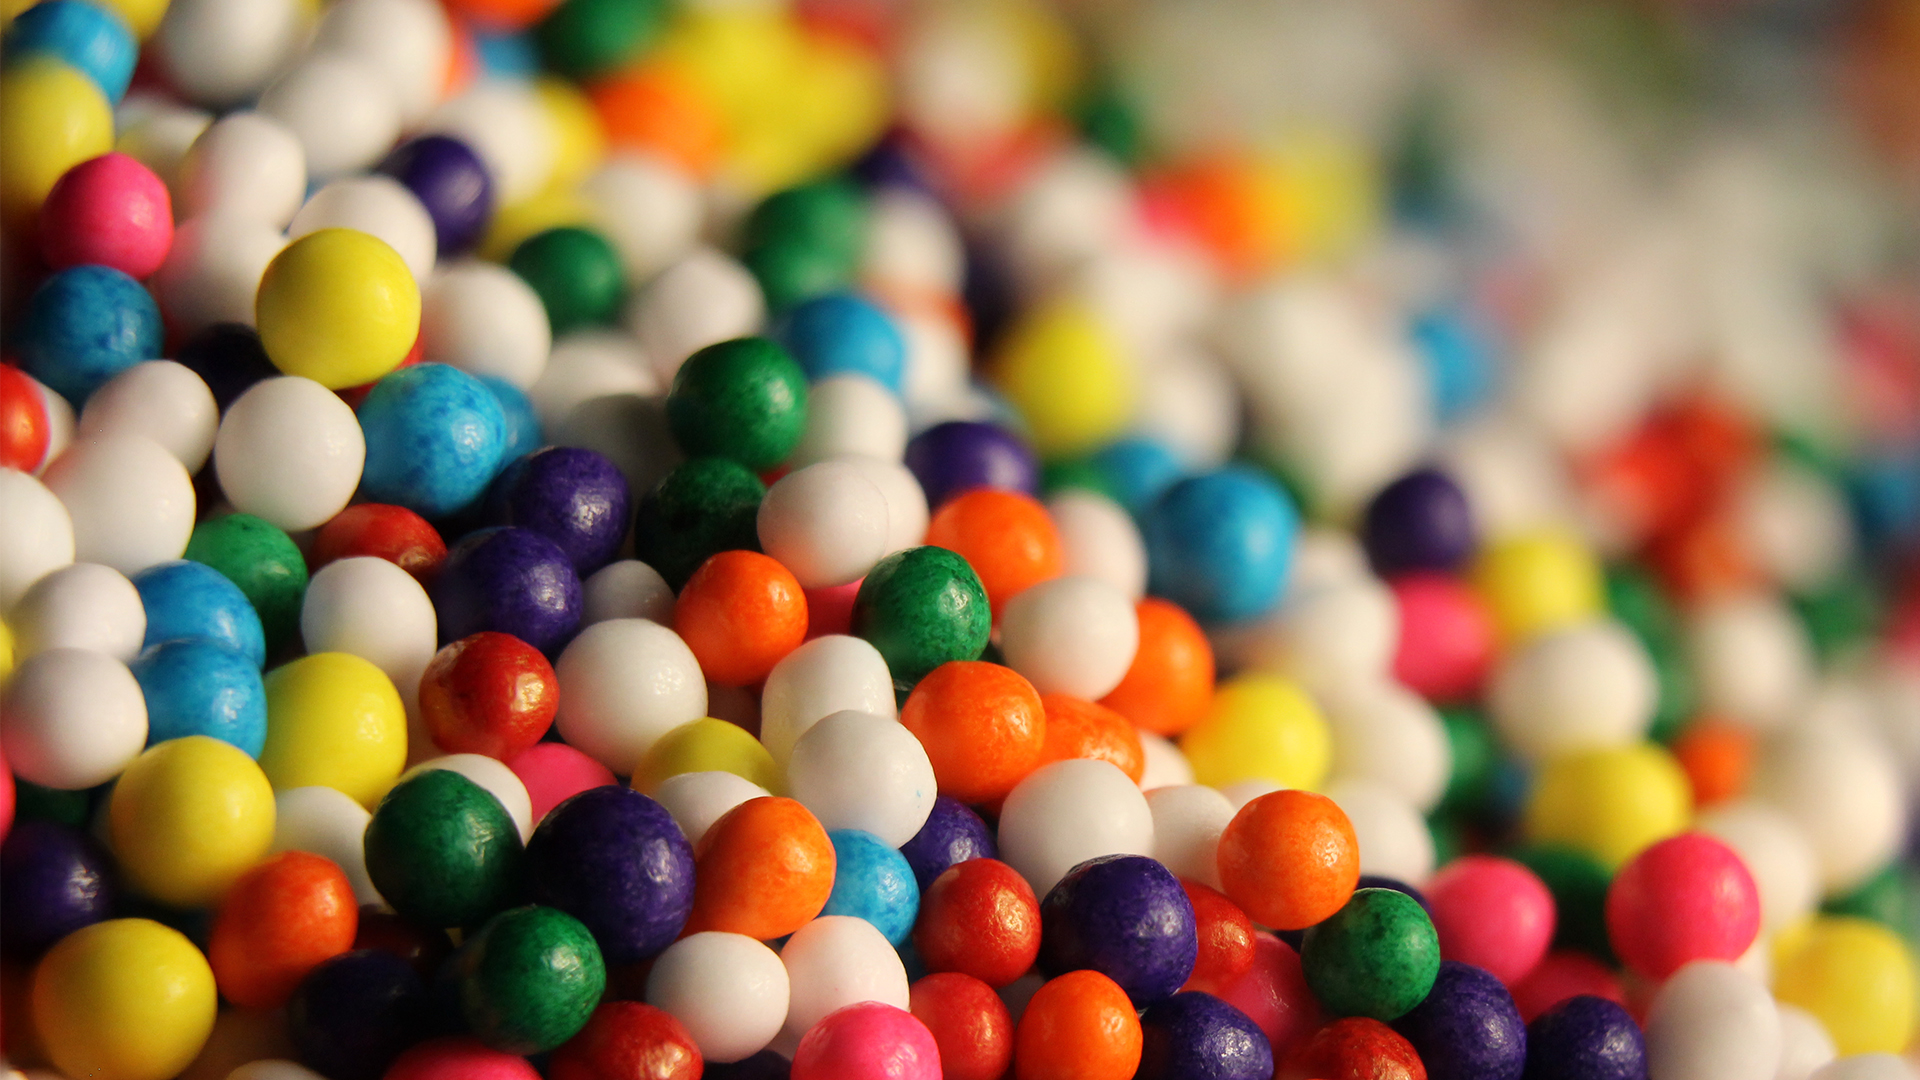
\includegraphics[width=100mm]{./figures/figure_example1.jpg}
%    \caption{图片测试(最小宽度)\\Image test (Minimal width)}
%  \end{figure}

\begin{figure}[H]
	\centering
	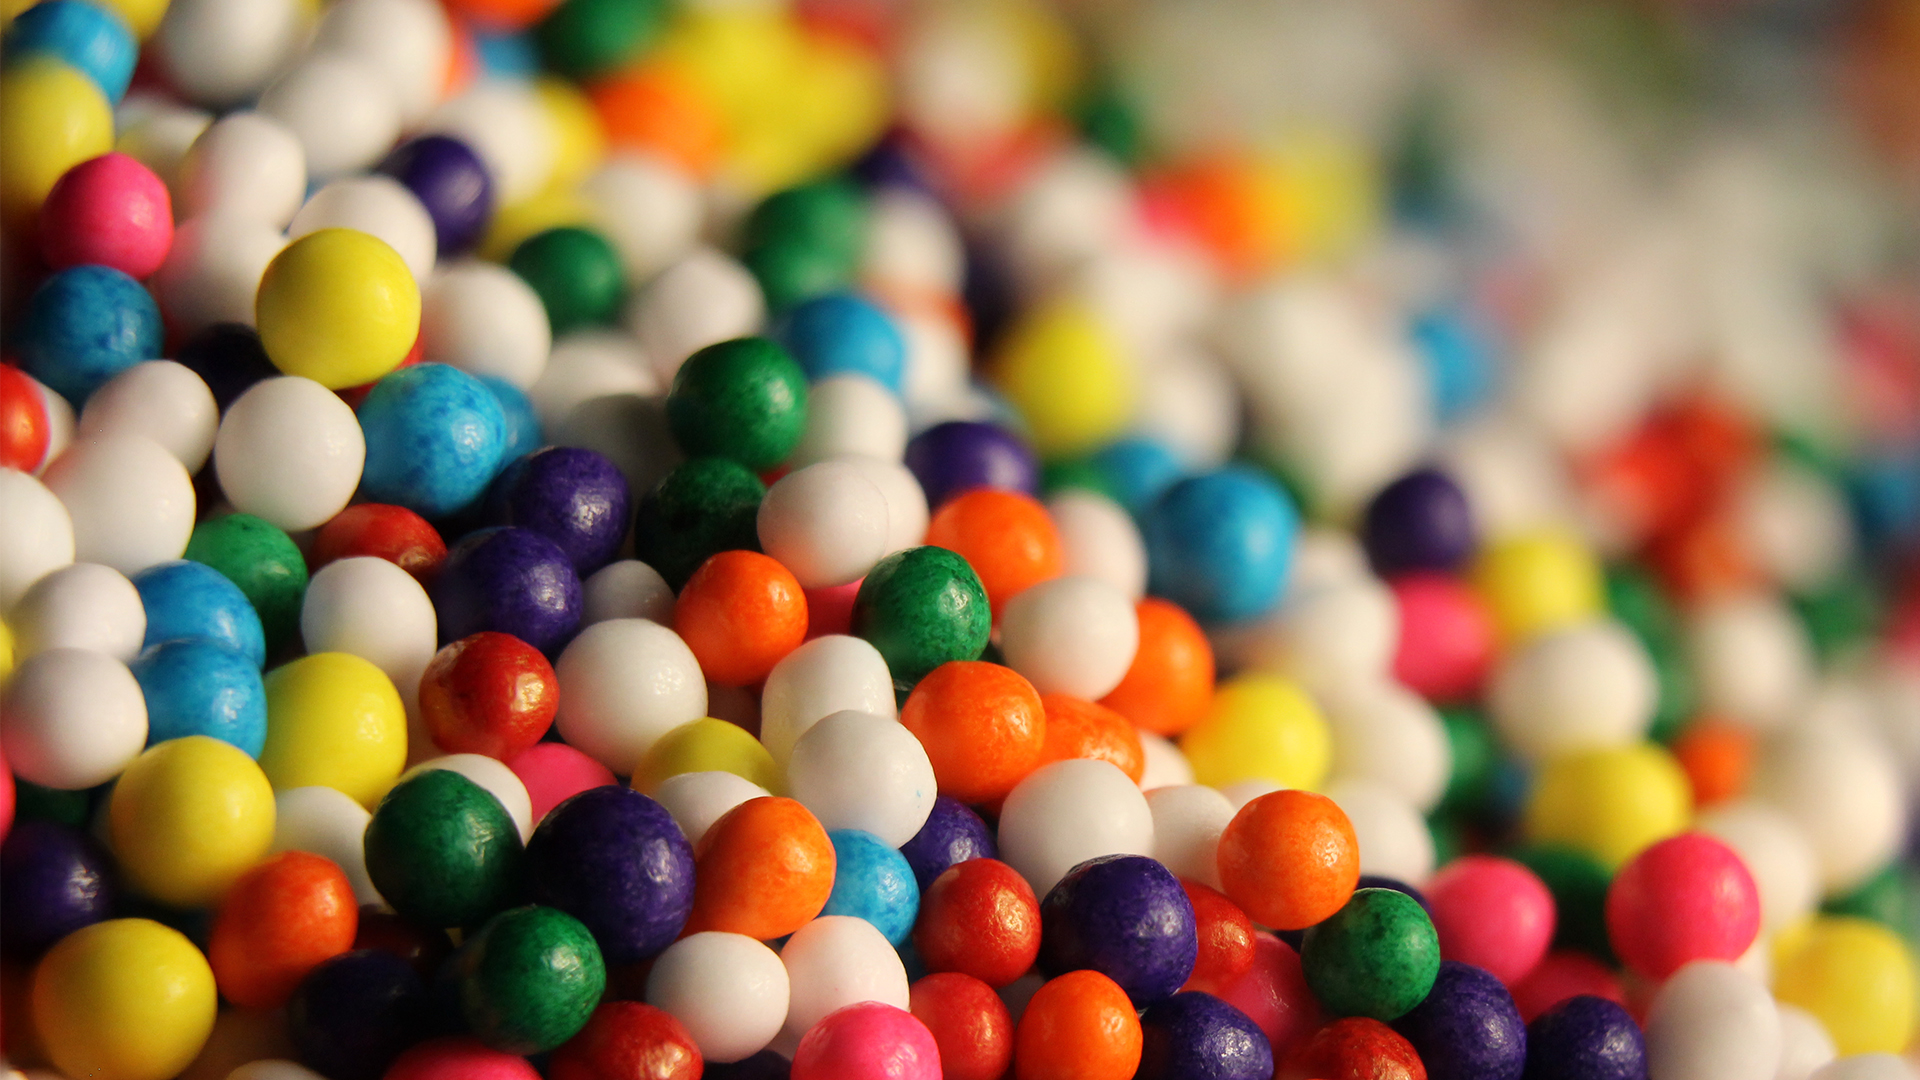
\includegraphics[width=0.3\linewidth]{./figures/figure_example1.jpg}
	\caption{ElegantLaTeX Logo}
	\label{fig:logo}
\end{figure}


%\begin{figure}[H]
%    \centering
%    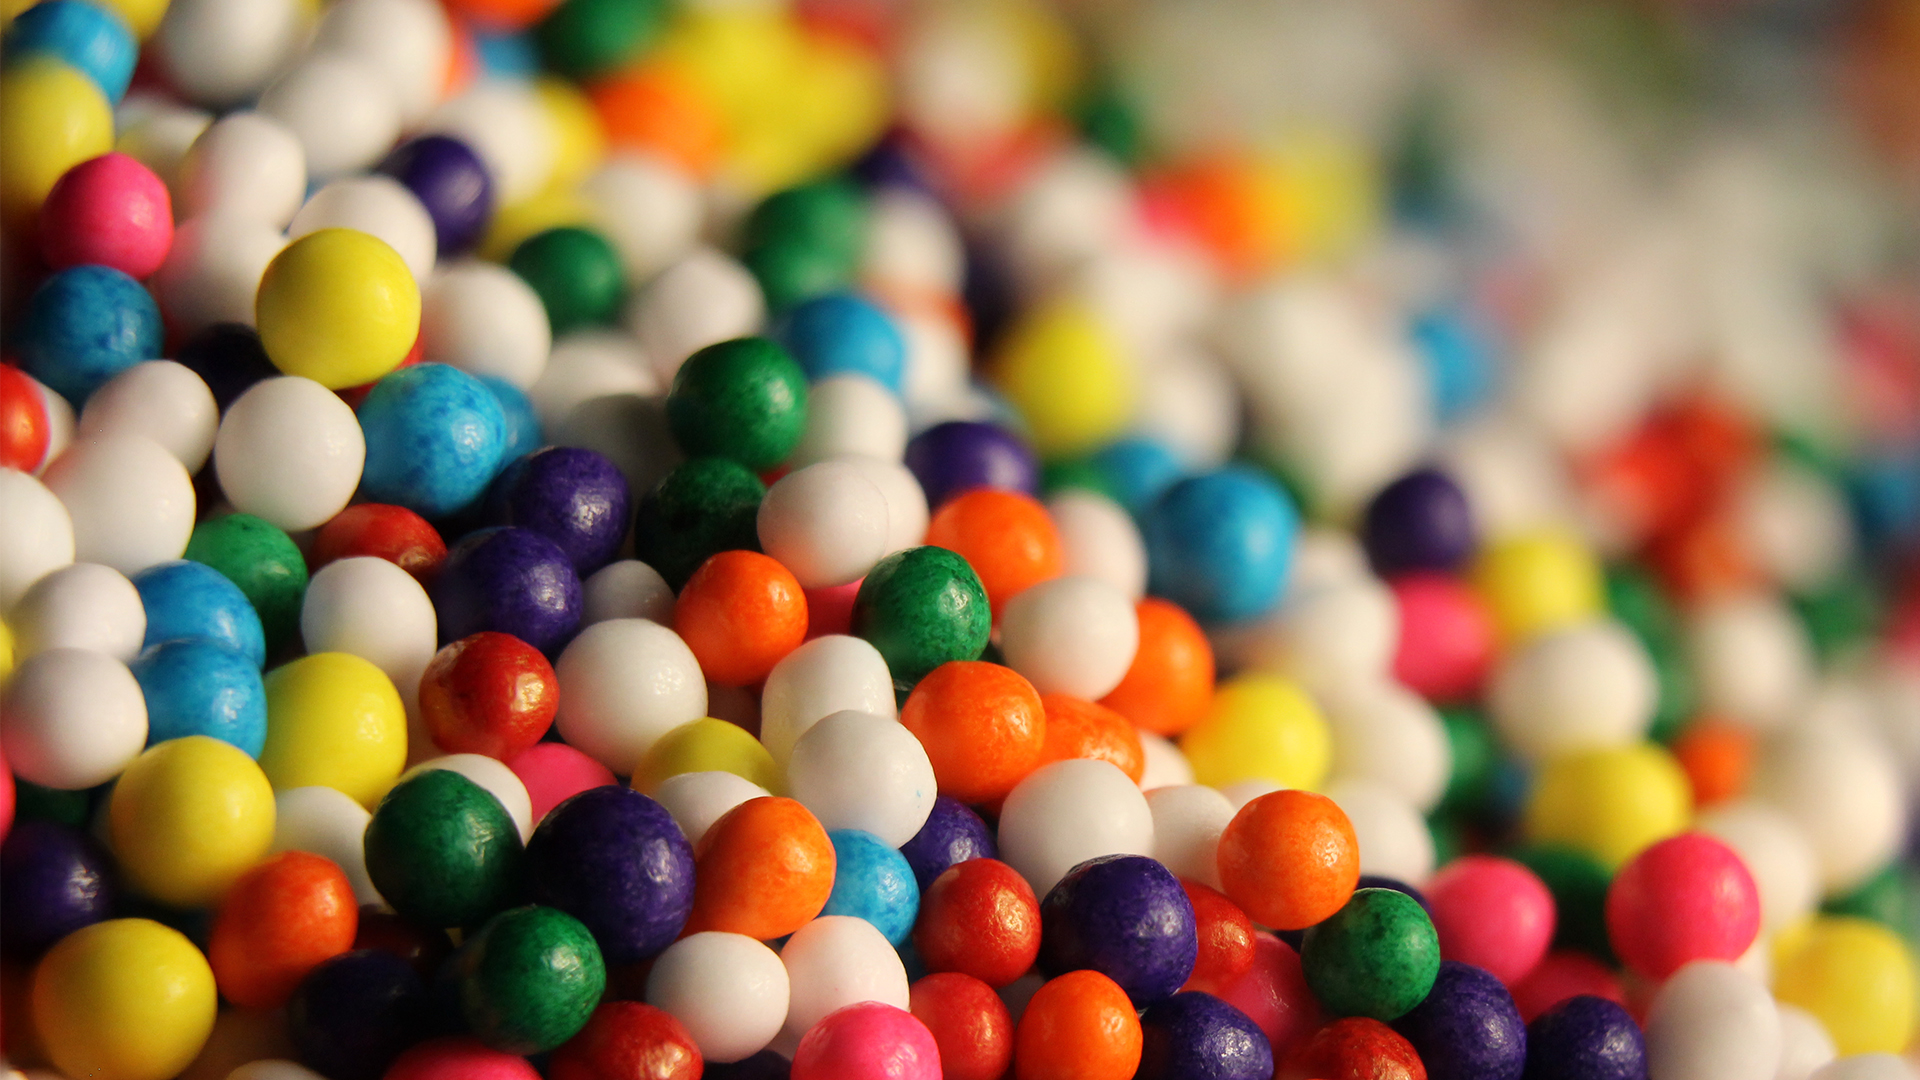
\includegraphics[width=130mm]{./figures/figure_example1.jpg}
%    \caption{图片测试(最大宽度)\\Image test (Maximal width)}
%\end{figure}
\par 注意:这里为了减少图片上下的空白,使用了float宏包。 %正文第四章  %
\clearpage                              %
%%%%%%%%%%%%%%%%%%%%%%%%%%%%%%%%%%%%%%%%%

\clearpage                              %
\section*{结论}                         %通常你不需要修改这部分内容
\addcontentsline{toc}{section}{结论}    %
这就是我的结论%倒入结论
\clearpage

\bibliographystyle{elsarticle-num-names}%参考文献按出场顺序排,plain按名字排列
\begin{thebibliography}{99}
	\bibitem{ul1} Haarmann H. Language in ethnicity: A view of basic ecological relations[M]. Walter de Gruyter, 1986.
	
	\bibitem{ul2} Landweer M L. Indicators of ethnolinguistic vitality[J]. Notes on sociolinguistics, 2000, 5(1): 5-22.
	
	\bibitem{ul3} Jarvis S. Conceptual transfer in the interlingual lexicon[M]. Indiana University Linguistics Club Publications, 1998.
	
	\bibitem{ul4} Talmy L. Toward a cognitive semantics[M]. MIT press, 2000.
	 
	\bibitem{ul5} Jarvis S, Pavlenko A. Crosslinguistic influence in language and cognition[M]. Routledge, 2008.
	
	\bibitem{ul6} The East Asian welfare model: Welfare orientalism and the state[M]. Psychology press, 1998.
	
	\bibitem{ul7} Lewis M P, Simons G F, Fennig C D. Ethnologue: Languages of the world[M]. Dallas, TX: SIL international, 2009.
	
	\bibitem{ul8} Kushner E. English as global language: problems, dangers, opportunities[J]. Diogenes, 2003, 50(2): 17-23.
	 
	\bibitem{ul9} Upchurch M. Sounding the Alarm about Extinction of World's Languages[J]. Seattle Times, 2000-08-27, 2000.
	
	\bibitem{ul10} Swain A D, Guttmann H E. Handbook of human-reliability analysis with emphasis on nuclear power plant applications. Final report[R]. Sandia National Labs., Albuquerque, NM (USA), 1983.
	 
	\bibitem{ul11} Moriarty M. Globalization and Minority-Language Policy and Planning[M]//Globalizing Language Policy and Planning. Palgrave Macmillan, London, 2015: 9-23.
	
\end{thebibliography}%你所需要的参考文献

\addcontentsline{toc}{section}{参考文献}  


\makeacknowledgement %生成感谢
%强制生成附录
\clearpage
\addcontentsline{toc}{section}{附录}
\makeapdx

\end{document}